\documentclass[portrait,a0paper]{baposter}
%\documentclass[a4shrink,portrait,final]{baposter}
% Usa a4shrink for an a4 sized paper.
%\tracingstats=2

\usepackage[utf8]{inputenc}
%\usepackage{fontspec}

\usepackage{calc}
\usepackage{graphicx}
\usepackage{amsmath}
\usepackage{amssymb}
\usepackage{relsize}
\usepackage{graphicx}
\usepackage{multirow}
\usepackage{multicol}
\usepackage{url}
\usepackage{microtype}
\usepackage{caption}

%\usepackage{pgfbaselayers}
\pgfdeclarelayer{background}
\pgfdeclarelayer{foreground}
\pgfsetlayers{background,main,foreground}

\usetikzlibrary{calc,arrows,decorations}
\usetikzlibrary{decorations.shapes}
\usetikzlibrary{decorations.pathreplacing}
\usetikzlibrary{decorations.markings}
\usetikzlibrary{shapes,arrows}
\usetikzlibrary{shadows}
\usetikzlibrary{patterns}
\usetikzlibrary{decorations.pathmorphing}

\usepackage{grffile}
\usepackage{carl_commands}

%\usepackage{times}
%\usepackage{helvet}
%\usepackage{bookman}
\usepackage{palatino}

%\newcommand{\captionfont}{\footnotesize}

\selectcolormodel{cmyk}

%%%%%%%%%%%%%%%%%%%%%%%%%%%%%%%%%%%%%%%%%%%%%%%%%%%%%%%%%%%%%%%%%%%%%%%%%%%%%%%%
%%%% Some math symbols used in the text
%%%%%%%%%%%%%%%%%%%%%%%%%%%%%%%%%%%%%%%%%%%%%%%%%%%%%%%%%%%%%%%%%%%%%%%%%%%%%%%%
% Format 
\newcommand{\Matrix}[1]{\begin{bmatrix} #1 \end{bmatrix}}
\newcommand{\Vector}[1]{\Matrix{#1}}
\newcommand*{\SET}[1]  {\ensuremath{\mathcal{#1}}}
\newcommand*{\MAT}[1]  {\ensuremath{\mathbf{#1}}}
\newcommand*{\VEC}[1]  {\ensuremath{\bm{#1}}}
\newcommand*{\CONST}[1]{\ensuremath{\mathit{#1}}}
\newcommand*{\norm}[1]{\mathopen\| #1 \mathclose\|}% use instead of $\|x\|$
\newcommand*{\abs}[1]{\mathopen| #1 \mathclose|}% use instead of $\|x\|$
\newcommand*{\absLR}[1]{\left| #1 \right|}% use instead of $\|x\|$

\def\norm#1{\mathopen\| #1 \mathclose\|}% use instead of $\|x\|$
\newcommand{\normLR}[1]{\left\| #1 \right\|}% use instead of $\|x\|$

%%%%%%%%%%%%%%%%%%%%%%%%%%%%%%%%%%%%%%%%%%%%%%%%%%%%%%%%%%%%%%%%%%%%%%%%%%%%%%%%
% Multicol Settings
%%%%%%%%%%%%%%%%%%%%%%%%%%%%%%%%%%%%%%%%%%%%%%%%%%%%%%%%%%%%%%%%%%%%%%%%%%%%%%%%
\setlength{\columnsep}{0.7em}
\setlength{\columnseprule}{0mm}

%%%%%%%%%%%%%%%%%%%%%%%%%%%%%%%%%%%%%%%%%%%%%%%%%%%%%%%%%%%%%%%%%%%%%%%%%%%%%%%%
% Save space in lists. Use this after the opening of the list
%%%%%%%%%%%%%%%%%%%%%%%%%%%%%%%%%%%%%%%%%%%%%%%%%%%%%%%%%%%%%%%%%%%%%%%%%%%%%%%%
\newcommand{\compresslist}{%
\setlength{\itemsep}{1pt}%
\setlength{\parskip}{0pt}%
\setlength{\parsep}{0pt}%
}

\renewcommand{\emph}[1]{\textcolor{chalmers_lightblue}{#1}}

%%%%%%%%%%%%%%%%%%%%%%%%%%%%%%%%%%%%%%%%%%%%%%%%%%%%%%%%%%%%%%%%%%%%%%%%%%%%%%
%%% Begin of Document
%%%%%%%%%%%%%%%%%%%%%%%%%%%%%%%%%%%%%%%%%%%%%%%%%%%%%%%%%%%%%%%%%%%%%%%%%%%%%%

\begin{document}

%%%%%%%%%%%%%%%%%%%%%%%%%%%%%%%%%%%%%%%%%%%%%%%%%%%%%%%%%%%%%%%%%%%%%%%%%%%%%%
%%% Here starts the poster
%%%---------------------------------------------------------------------------
%%% Format it to your taste with the options
%%%%%%%%%%%%%%%%%%%%%%%%%%%%%%%%%%%%%%%%%%%%%%%%%%%%%%%%%%%%%%%%%%%%%%%%%%%%%%
% Define some colors
\definecolor{chalmers_blue}     {RGB}{  0,  0,102}
\definecolor{chalmers_grey}     {RGB}{204,204,204}
\definecolor{chalmers_lightblue}{RGB}{ 28, 78,157}%{1c4e9d}
\definecolor{chalmers_lightblue}{cmyk}{0.9,0.60,0.0,0.2}
%\definecolor{chalmers_lightblue}{RGB}{50, 150, 250}%{1c4e9d}
\definecolor{chalmers_lightgold}{RGB}{239,197, 22}%{efc516}
\definecolor{chalmers_purple}   {RGB}{ 51, 51,102}%{333366}

%%
\typeout{Poster Starts}
\background{
  \begin{tikzpicture}[remember picture,overlay]%
    %\draw (current page.north west)+(-2em,2em) node[anchor=north west] {\includegraphics[height=1.1\textheight]{silhouettes_background}};
  \end{tikzpicture}%
}

\newlength{\leftimgwidth}
\begin{poster}%
  % Poster Options
  {
  % Show grid to help with alignment
  grid=no,
  % Column spacing
  colspacing=1em,
  % Color style
  bgColorOne=white,
  bgColorTwo=white,
  borderColor=chalmers_lightblue,
  headerColorOne=chalmers_lightblue,
  headerFontColor=white,
  boxColorOne=white,
  % Format of textbox
  textborder=faded,
  % Format of text header
  eyecatcher=no,
  headerborder=open,
  headerheight=0.08\textheight,
  headershape=roundedright,
  headershade=plain,
  headerfont=\Large\textsc, %Sans Serif
  boxshade=plain,
  %background=shade-tb,
  background=plain,
  linewidth=2pt
  }
  % Eye Catcher
  {\includegraphics[width=10em]{D1077}} % eye catcher
  % Title
  {\scshape OOFEM:\\development platform for FE research}
  % Authors
  {\vspace{0.5em}Mikael Öhman, \url{mikael.ohman@chalmers.se}\\[-0.5em]\small Department of Applied Mechanics, Chalmers University of Technology}
  % University logo
  {% The makebox allows the title to flow into the logo, this is a hack because of the L shaped logo.
  \begin{tabular}{c}
    
\includegraphics[width=5em]{figures/Avancez_black}\\
    \raisebox{0em}[0em][0em]{
\includegraphics[width=9em]{figures/CHALMERS_black}}
  \end{tabular}
  }

  % Width of left inset image
     \setlength{\leftimgwidth}{0.78em+8.0em}

%%%%%%%%%%%%%%%%%%%%%%%%%%%%%%%%%%%%%%%%%%%%%%%%%%%%%%%%%%%%%%%%%%%%%%%%%%%%%%
  \headerbox{Example 1: Multiscale modeling of viscous sintering}{name=mikael,row=0,column=1,span=2}{
%%%%%%%%%%%%%%%%%%%%%%%%%%%%%%%%%%%%%%%%%%%%%%%%%%%%%%%%%%%%%%%%%%%%%%%%%%%%%%
The macroscale is a volumetrically compressible problem, characterized by a varying density in a green body (compressed powder).
In contrast, the subscale is modeled as a incompressible free surface Stokes flow, driven by surface tension.

For the macroscale, a straight forward implementation of the momentum-balance equation is used, coupled to the micro problems through the Gauss points. 

In the subscale, surface tension is modeled by \emph{specialized surface elements}. For the free surface flow, a \emph{Grid Base Particle Method} (GBPM) is implemented for tracking the active surface. Updating the velocities means finding elements using an \emph{Octree based localizer}.
Remeshing is done with \emph{Triangle} whenever the mesh quality drops too low or whenever large topological changes occur. 

The prolongation for the Dirichlet boundary conditions were implemented with a specialized boundary condition for \emph{prescribed gradients}.
Using these structures, the computational homogenization was written in a few simple lines of code.
\vspace{-0.5em}
\begin{center}
 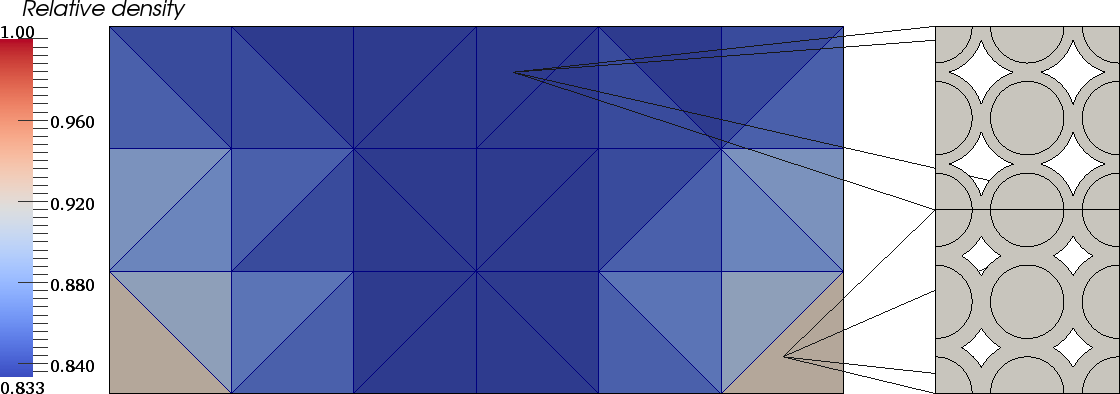
\includegraphics[width=0.8\linewidth]{figures/macro_sintering_2x2.0000.png}
 \captionof{figure}{Multiscale computations at $t = t_{\text{start}}$}
\end{center}
\vspace{-2em}
\begin{center}
 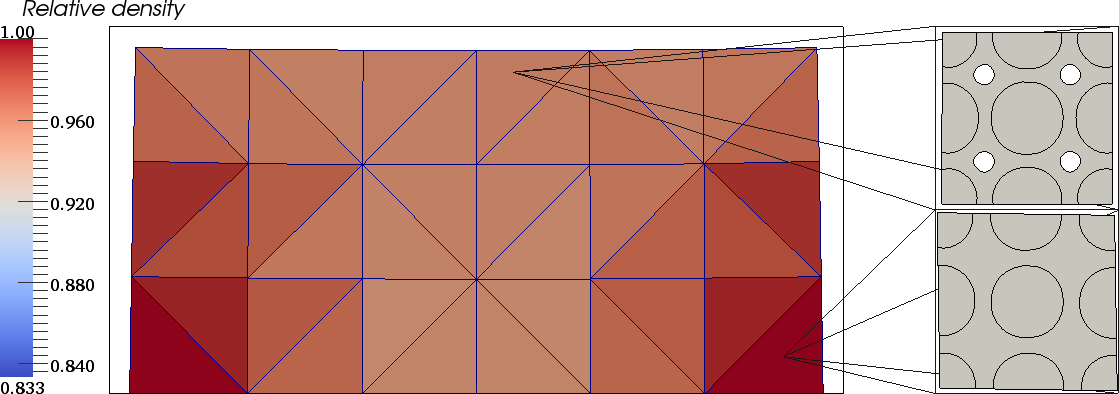
\includegraphics[width=0.8\linewidth]{figures/macro_sintering_2x2.0176.png}
 \captionof{figure}{Multiscale computations at $t = t_{\text{end}}$}
\end{center}
\vspace{-0.5em}
\textit{Example by Mikael Öhman. Presented on Tuesday, Session Flerfarströmning II, 11:35.}
  }

%%%%%%%%%%%%%%%%%%%%%%%%%%%%%%%%%%%%%%%%%%%%%%%%%%%%%%%%%%%%%%%%%%%%%%%%%%%%%%
  \headerbox{Example 2: Multiscale modeling of creeping flow}{name=carl,column=1,span=2,below=mikael,above=bottom}{
%%%%%%%%%%%%%%%%%%%%%%%%%%%%%%%%%%%%%%%%%%%%%%%%%%%%%%%%%%%%%%%%%%%%%%%%%%%%%%

      \begin{multicols}{2}
The macroscale problem is a creeping flow, and the microscale is described by a incompressible Stokes flow.

The coupled FE\textsuperscript{2} problem has been implemented in OOFEM in the heat transfer and fluid mechanics module respectively.
For the microscale problem, the periodic boundary conditions are implemented using \emph{slave DOF's}.

The nonlinear system of equations are solved with \emph{line-search}.
        \columnbreak
        \begin{center}
        \begin{tikzpicture}[scale=0.7]
        \input{figures/carl/MacroDomainFilter.tex}
        \end{tikzpicture}
        \end{center}
      \end{multicols}\vspace{-1em}
      \mbox{\hspace{0.3\linewidth}\rule{0.4\linewidth}{1pt}\hspace{0.3\linewidth}}\\
      \vspace{-2em}
	  \begin{center}
	  \begin{tikzpicture}[scale=0.5]
	  \input{figures/carl/NumericalExampleResult.tex}
	  \end{tikzpicture}
      \captionof{figure}{Results from a fully coupled nonlinear FE\textsuperscript{2} simulation}
	  \end{center}

\textit{Example by Carl Sandström. Presented on Tuesday, Session Materialmodellering II, 16:35.}
  }

%%%%%%%%%%%%%%%%%%%%%%%%%%%%%%%%%%%%%%%%%%%%%%%%%%%%%%%%%%%%%%%%%%%%%%%%%%%%%%
  \headerbox{Development}{name=development,column=0,row=0,span=1}{
%%%%%%%%%%%%%%%%%%%%%%%%%%%%%%%%%%%%%%%%%%%%%%%%%%%%%%%%%%%%%%%%%%%%%%%%%%%%%%
   \begin{itemize}\setlength{\itemsep}{0.05em}
    \item C++ with Python Bindings
    \item Object-Oriented
    \item Well documented
    \begin{itemize}
     \item Doxygen
     \item Input file documentation
    \end{itemize}
    \item Fully extensible
    \item Flexible interface structure
    \item Automatic test suite
    \item GPLv2 license
   \end{itemize}
    \begin{minipage}[t]{0.3\linewidth}
     \begin{itemize}\setlength{\itemsep}{0.05em}
     \item Trac
     \item SVN
    \end{itemize}
    \end{minipage}
    \begin{minipage}[t]{0.6\linewidth}
    \begin{itemize}\setlength{\itemsep}{0.05em}
     \item Forums and Wiki
     \item Ohloh
     \end{itemize}
    \end{minipage}
   \\[1em]
   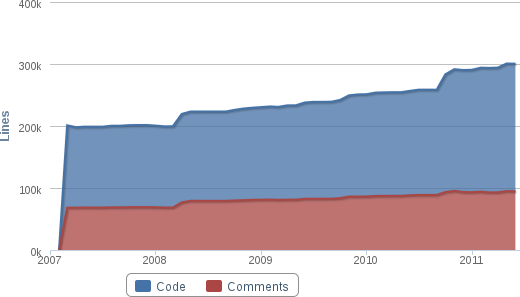
\includegraphics[width=\linewidth]{figures/ohloh}
   More information at: \textcolor{blue}{\textbf{\url{www.oofem.org}}}
  }

%%%%%%%%%%%%%%%%%%%%%%%%%%%%%%%%%%%%%%%%%%%%%%%%%%%%%%%%%%%%%%%%%%%%%%%%%%%%%%
  \headerbox{Features}{name=features,column=0,below=development}{
%%%%%%%%%%%%%%%%%%%%%%%%%%%%%%%%%%%%%%%%%%%%%%%%%%%%%%%%%%%%%%%%%%%%%%%%%%%%%%
   \begin{itemize}\setlength{\itemsep}{0.05em}
     \item Convenient routines for:
    \begin{itemize}
     \item Dense and sparse linear algebra
     \item Interpolation and integration
     \item Spatial search algorithms
     \item Variable mapping
     \item Quality measurement
     \item[\ldots]
    \end{itemize}
    \item Familiar open source connections
    \begin{itemize}
     \item PETSc
     \item VTK
     \item BLAS/LAPACK
     \item[\ldots]
    \end{itemize}
    \item Fluid-, Solid mechanics and heat transfer solvers
    \item Adaptivity
    \item X-FEM
    \item Full restart
    \item Parallel processing
    \item Iso-Geometric Analysis
   \end{itemize}

  }

%%%%%%%%%%%%%%%%%%%%%%%%%%%%%%%%%%%%%%%%%%%%%%%%%%%%%%%%%%%%%%%%%%%%%%%%%%%%%%
  \headerbox{Planned Features}{name=upcoming,column=0,below=features}{
%%%%%%%%%%%%%%%%%%%%%%%%%%%%%%%%%%%%%%%%%%%%%%%%%%%%%%%%%%%%%%%%%%%%%%%%%%%%%%
   \begin{itemize}\setlength{\itemsep}{0.05em}
    \item Active boundary conditions
    \item Compressed VTK
    \item Particle-FEM
    \item MATLAB/NumPy export.
   \end{itemize}
  }

%%%%%%%%%%%%%%%%%%%%%%%%%%%%%%%%%%%%%%%%%%%%%%%%%%%%%%%%%%%%%%%%%%%%%%%%%%%%%%
  \headerbox{Contributors}{name=contributors,column=0,below=upcoming,above=bottom}{
%%%%%%%%%%%%%%%%%%%%%%%%%%%%%%%%%%%%%%%%%%%%%%%%%%%%%%%%%%%%%%%%%%%%%%%%%%%%%%
   Developed at Czech Technical University in Prague, with contributions from many other Universities.
  }


\end{poster}

\end{document}
